\documentclass[conference]{IEEEtran}
\usepackage[utf8]{inputenc}
\usepackage[T1]{fontenc}
\usepackage[brazilian]{babel}
\usepackage{cite}
\usepackage{amsmath,amssymb,amsfonts}
\usepackage{graphicx}
\usepackage{textcomp}
\usepackage{xcolor}
\usepackage{url}
\usepackage{booktabs}
\usepackage{array}
\usepackage{placeins}

\renewcommand{\refname}{Referências}
\renewcommand{\tablename}{Tabela}
\renewcommand{\figurename}{Fig.}
\newcommand{\svm}{\mbox{SVM-RBF}}
\raggedbottom

\begin{document}

\title{Kernel quântico versus SVM clássico ajustado sobre embeddings comprimidos: classificação de sentimentos em português e inglês}

\author{\IEEEauthorblockN{Júlia Alves}
\IEEEauthorblockA{\textit{Ciência da Computação} \\
\textit{Inteli, Instituto de Tecnologia e Liderança}\\
São Paulo, Brasil \\
julia.jesus@sou.inteli.edu.br}
\and
\IEEEauthorblockN{Erinaldo Fonseca e Bryan Ferreira}
\IEEEauthorblockA{\textit{Orientadores} \\
\textit{Inteli, Instituto de Tecnologia e Liderança}\\
São Paulo, Brasil}
}

\maketitle

\renewcommand{\abstractname}{Resumo}
\renewcommand{\IEEEkeywordsname}{Palavras-chave}
\begin{abstract}
Classificadores baseados em kernel dependem de uma medida que diz o quanto dois exemplos se parecem, e os kernels quânticos aparecem como uma forma diferente de calcular essa similaridade, inclusive para embeddings de frases, que precisam ser comprimidos para caber em poucos qubits. Nos trabalhos que testam esse tipo de classificador, porém, a comparação com modelos clássicos costuma ser feita em condições diferentes, o que dificulta entender de onde vem a diferença entre eles. Este trabalho compara um QSVM com kernel quântico de fidelidade a classificadores clássicos que recebem exatamente as mesmas features comprimidas, com busca de hiperparâmetros aninhada para todos os modelos, usando a base Yelp, em inglês, e a RePro, em português. No cenário de estado exato, o QSVM com a largura de banda ajustada chegou a valores de F1-macro entre 0,91 e 0,95, no mesmo patamar dos modelos clássicos, e não foi detectada diferença estatisticamente significativa em relação a eles em nenhuma das 12 configurações. Com largura de banda fixa, o QSVM ficou perto de 0,50 no teste e, com 8 e 12 qubits, decorou o treino, e a versão do circuito sem emaranhamento teve desempenho semelhante ao da versão com emaranhamento. Os resultados não mostram vantagem do kernel quântico nesse cenário de comparação e indicam que o desempenho dele depende principalmente do ajuste da largura de banda.
\end{abstract}

\begin{IEEEkeywords}
aprendizado de máquina quântico, kernel quântico, embeddings de sentenças, análise de sentimentos, português
\end{IEEEkeywords}

\renewcommand{\abstractname}{Abstract}
\renewcommand{\IEEEkeywordsname}{Keywords}
\begin{abstract}
Kernel-based classifiers depend on a measure of how similar two examples are, and quantum kernels appear as a different way to compute this similarity, including for sentence embeddings, which need to be compressed to fit into a few qubits. In studies that test this kind of classifier, however, the comparison with classical models is often made under different conditions, which makes it difficult to understand where the difference between them comes from. This work compares a QSVM with a fidelity quantum kernel to classical classifiers that receive exactly the same compressed features, with nested hyperparameter search for all models, using the Yelp dataset, in English, and RePro, in Portuguese. In the exact-state scenario, the QSVM with a tuned bandwidth reached macro-F1 values between 0.91 and 0.95, at the same level as the classical models, and no statistically significant difference from them was detected in any of the 12 configurations. With a fixed bandwidth, the QSVM stayed close to 0.50 on the test set and, with 8 and 12 qubits, memorized the training set, and the circuit without entanglement performed similarly to the entangled one. The results show no detected advantage for the quantum kernel in this comparison and indicate that its performance depends mainly on tuning the bandwidth.
\end{abstract}

\begin{IEEEkeywords}
quantum machine learning, quantum kernels, sentence embeddings, sentiment analysis, Portuguese
\end{IEEEkeywords}

\section{Introdução}

Atualmente, boa parte das tarefas de classificação de texto, como a análise de sentimento de avaliações de produtos, é feita com modelos de linguagem que representam palavras e frases por meio de embeddings. Nesses embeddings, cada frase vira um vetor numérico e, nesse espaço vetorial, frases com sentido parecido tendem a ficar mais próximas, o que pode ser medido, por exemplo, pela similaridade de cosseno \cite{reimers2019}. Boa parte dos classificadores usados em cima desses vetores, como os que usam kernels, depende justamente de uma medida desse tipo, que diz o quanto dois exemplos se parecem. Com isso, surgem soluções na computação quântica que propõem outra forma de calcular essa similaridade, como os kernels quânticos, em que ela é obtida a partir de estados quânticos \cite{havlicek2019}.

O desafio vem de entender quais as limitações e o que é perdido durante o processo de representação e compressão das frases, já que um embedding de frase tem centenas de dimensões, enquanto os circuitos que é possível simular hoje trabalham com poucos qubits, então as frases precisam ser comprimidas antes de chegar no circuito e o modelo quântico acaba recebendo uma versão reduzida delas. Bowles et al. \cite{bowles2024} comentam que esse tipo de pré-processamento pode mudar a dificuldade e até a natureza do problema, olhando para benchmarks de imagens, e Hassan et al. \cite{hassan2026}, já em classificação de texto, mostram quanto da variância o PCA consegue manter e como a acurácia muda depois da compressão. Isso deixa a comparação entre modelos quânticos e clássicos mais delicada, e no mesmo trabalho Bowles et al. mostram que cerca de 40\% de uma amostra de 55 artigos selecionados por eles afirma que o modelo quântico supera o clássico, mas, quando testaram 12 modelos quânticos em 160 conjuntos de dados, os modelos clássicos se saíram melhor no geral. Em modelos híbridos, que misturam partes clássicas e quânticas, Kölle et al. \cite{kolle2024} também perceberam que a parte clássica costuma fazer boa parte do trabalho, mesmo quando o mérito acaba sendo dado para a parte quântica.

Ao olhar para texto, esse problema também aparece em vários trabalhos. Hassan et al. \cite{hassan2026} comprimem embeddings de sentenças antes de usar um classificador quântico variacional (VQC) em uma tarefa de classificação de perguntas, mas comparam o resultado com um modelo clássico que usou os dados sem compressão, e os próprios autores comentam que ainda falta comparar os dois em cima das mesmas representações. Cajas Ordóñez et al. \cite{cajas2025} afirmam ter um ganho relativo de até 8\% com o kernel quântico, com a acurácia indo de 0,833 para 0,900, porém em embeddings de imagens e contra um SVM com hiperparâmetros fixos, enquanto Djemmal et al. \cite{djemmal2025} propõem uma compressão pensada para o circuito quântico, mas o QNN que eles usam como referência, sem a compressão proposta, fica perto de 50\% de acurácia, com precisão de cerca de 0,24 e recall de 0,50 em duas das três bases, o que indica que ele prevê praticamente uma classe só. Nesse caso, fica difícil dizer se o problema vem dos circuitos, de um comparativo base fraco, da compressão ou de outras razões.

Ainda pensando nas limitações que essas soluções com computação quântica apresentam, existe outra preocupação no que diz respeito à escalabilidade, ou seja, ao que acontece com o kernel conforme o número de qubits vai aumentando, já que Thanasilp et al. \cite{thanasilp2024} mostram que, sob certas condições, os valores do kernel tendem a ficar muito parecidos entre si conforme os qubits aumentam, e as diferenças entre eles ficam tão pequenas que é preciso um número cada vez maior de medições para conseguir diferenciar um exemplo do outro. Por outro lado, Shaydulin e Wild \cite{shaydulin2021} mostram que boa parte desse efeito está ligada à largura de banda do kernel, que é um fator de escala aplicado aos dados antes do circuito, e que, quando ela é ajustada, o desempenho pode até melhorar com mais qubits. Na literatura, Maio \cite{maio2026}, em um trabalho sobre embeddings quantum-inspired, também testou um kernel quântico simulado sobre embeddings de texto em uma tarefa de recuperação, mas com um número fixo de 12 qubits e sem testar classificação. Algumas das diferenças encontradas na revisão bibliográfica sobre o assunto dizem respeito à forma como os modelos quânticos e clássicos são comparados e à falta de testes desse efeito em classificação, além do uso de bases que não estão em língua portuguesa.

Assim, o problema que motiva este trabalho é a falta de uma comparação entre classificadores quânticos e clássicos feita sobre as mesmas representações comprimidas de texto e com o comparativo base ajustado, o que impede saber se o desempenho relatado para kernels quânticos vem do circuito ou das condições em que a comparação foi feita. Com o propósito de resolver essa lacuna, este trabalho busca comparar o desempenho de um QSVM com kernel quântico de fidelidade ao de classificadores clássicos ajustados que recebem exatamente as mesmas representações comprimidas de textos em português e inglês, identificando como o ajuste do comparativo base, o tipo de compressão e o número de qubits afetam essa comparação. A pergunta principal deste trabalho é se, em embeddings de sentenças comprimidos para 4, 8 e 12 dimensões, um QSVM com kernel de fidelidade apresenta F1-macro diferente de um \svm{} ajustado pelo mesmo procedimento e treinado sobre as mesmas features. A partir dela, o trabalho também busca responder se essa diferença muda quando o \svm{} usa a configuração padrão, se ela muda conforme a compressão usa ou não os rótulos, como os valores do kernel se comportam com o aumento do número de qubits, com largura de banda fixa e ajustada, e se o emaranhamento do circuito contribui para o resultado.

Para isso, são usadas uma base de avaliações em inglês, a Yelp \cite{kotzias2015}, e outra em português, a RePro \cite{repro2024}, que foi construída a partir do corpus B2W-Reviews01 \cite{real2019}. Como a RePro tem quatro rótulos (positivo, negativo, neutro e positivo/negativo, para avaliações mistas) e a Yelp é binária, da RePro são mantidas só as avaliações positivas e negativas, com 500 de cada classe, igual à Yelp, e a seleção também prioriza avaliações de tamanho próximo ao das frases da Yelp. Mesmo assim, as duas bases continuam diferentes em mais do que a língua, já que a Yelp tem frases soltas sobre restaurantes e a RePro tem avaliações de produtos, então o português não é tratado aqui como um fator comparado, e sim como um teste de generalização, no sentido de repetir a mesma comparação em outra base, e não de treinar em uma base e testar na outra. A ideia é ver se o que acontece na Yelp se repete em outra língua e em outro domínio, e, por isso, os modelos são sempre comparados dentro de cada base, nunca entre elas. Além disso, o SVM clássico é testado com a configuração padrão e também ajustado, para ver se a diferença entre os modelos muda com isso, e o QSVM passa pelo mesmo procedimento de ajuste, incluindo a largura de banda do kernel, para que a comparação não fique injusta para nenhum dos lados.

As principais contribuições deste trabalho são:
\begin{itemize}
\item comparar kernel quântico e modelos clássicos sobre as mesmas features comprimidas, com textos em português e em inglês, o que não foi encontrado em português na revisão realizada;
\item mostrar se o ajuste dos hiperparâmetros do SVM muda o resultado dessa comparação;
\item verificar se usar ou não os rótulos na compressão dos embeddings muda essa comparação;
\item observar o que acontece com o kernel quântico quando o número de qubits aumenta, agora em uma tarefa de classificação de texto, separando largura de banda fixa e ajustada e a simulação exata da estimativa com medições finitas.
\end{itemize}

No restante do artigo, a Seção~\ref{sec:desenho} apresenta as hipóteses; a Seção~\ref{sec:fundamentacao}, a fundamentação teórica; a Seção~\ref{sec:revisao}, a revisão bibliográfica; a Seção~\ref{sec:metodologia}, a metodologia, os parâmetros e as métricas; a Seção~\ref{sec:resultados}, os resultados; a Seção~\ref{sec:discussao}, a discussão, com a análise das hipóteses, a comparação com os trabalhos relacionados e as limitações; a Seção~\ref{sec:conclusao}, a conclusão e os trabalhos futuros; e a Seção~\ref{sec:codigo}, a organização dos códigos e dados.

\section{Desenho da pesquisa}
\label{sec:desenho}

Para responder à pergunta principal e às perguntas que vêm dela, o estudo foi organizado em seis hipóteses, uma para cada fator do desenho. H\textsubscript{0} e H\textsubscript{1} tratam da comparação principal; H\textsubscript{2} e H\textsubscript{3}, do efeito do comparativo base e da compressão; H\textsubscript{4}, do número de qubits; e H\textsubscript{5}, do papel do emaranhamento.

\begin{itemize}
\item \textbf{H\textsubscript{0}:} no cenário de estado exato, não há diferença estatisticamente significativa de F1-macro entre o QSVM e o \svm{} ajustado em nenhuma configuração.
\item \textbf{H\textsubscript{1}:} no cenário de estado exato, há diferença estatisticamente significativa de F1-macro entre o QSVM e o \svm{} ajustado em pelo menos uma configuração.
\item \textbf{H\textsubscript{2}:} a diferença de F1-macro a favor do QSVM é maior quando o \svm{} usa a configuração padrão do que quando ele é ajustado. A direção vem de Cajas Ordóñez et al. \cite{cajas2025}, que relatam ganho do kernel quântico justamente contra um SVM com C = 1 e gamma automático; se parte desse ganho vier do comparativo base fraco, ele deve diminuir quando o SVM é ajustado.
\item \textbf{H\textsubscript{3}:} a magnitude da diferença entre o QSVM e o \svm{} ajustado é menor quando a compressão usa os rótulos (NCA) do que quando não usa (PCA), já que a compressão supervisionada tende a deixar as classes mais separadas para qualquer modelo \cite{hassan2026}.
\item \textbf{H\textsubscript{4}:} no circuito e no protocolo usados, com largura de banda fixa, a variância dos valores do kernel fora da diagonal diminui com o aumento do número de qubits e o F1-macro cai junto; com largura de banda ajustada, essa queda é menor \cite{thanasilp2024,shaydulin2021}.
\item \textbf{H\textsubscript{5}:} o QSVM com emaranhamento não supera de forma significativa a versão do mesmo circuito sem as portas ZZ. A ausência de diferença significativa não demonstra equivalência entre os circuitos.
\end{itemize}

\section{Fundamentação teórica}
\label{sec:fundamentacao}

\subsection{Embeddings de sentenças}
Um embedding de sentença é um vetor numérico que representa o sentido de uma frase inteira. No Sentence-BERT \cite{reimers2019}, uma rede baseada no BERT é treinada para que frases com sentido parecido fiquem próximas, e essa proximidade costuma ser medida pela similaridade de cosseno, $\cos(\mathbf{u},\mathbf{v}) = \mathbf{u}\cdot\mathbf{v} / (\lVert\mathbf{u}\rVert\,\lVert\mathbf{v}\rVert)$. As versões multilíngues desses modelos são treinadas por destilação de conhecimento, de forma que uma frase e a sua tradução fiquem em pontos próximos do mesmo espaço \cite{reimers2020}, o que permite usar o mesmo modelo para o português e para o inglês.

\subsection{Redução de dimensionalidade}
Como os embeddings têm centenas de dimensões e cada dimensão vira um qubit no circuito, é preciso reduzir esses vetores antes. A análise de componentes principais (PCA) projeta os dados nas direções de maior variância, sem olhar para os rótulos \cite{jolliffe2002}, o que significa que a direção que separa as classes pode acabar sendo descartada se ela não tiver muita variância. Já a análise de componentes de vizinhança (NCA) aprende uma projeção linear usando os rótulos, escolhida para que cada exemplo fique perto de exemplos da mesma classe \cite{goldberger2004}, ou seja, é uma compressão supervisionada.

\subsection{SVM e kernels}
A máquina de vetores de suporte (SVM) encontra a fronteira que separa as classes com a maior margem possível \cite{cortes1995}. Ela não precisa dos vetores em si, só de uma função $k(\mathbf{x},\mathbf{x}')$ que mede a similaridade entre pares de exemplos, chamada de kernel. No kernel RBF, $k(\mathbf{x},\mathbf{x}') = \exp(-\gamma\lVert\mathbf{x}-\mathbf{x}'\rVert^2)$, o parâmetro $\gamma$ controla o quanto a similaridade cai com a distância, e o parâmetro C controla o quanto o modelo aceita errar no treino, então os dois precisam ser ajustados.

\subsection{Kernel quântico de fidelidade}
No kernel quântico, cada exemplo $\mathbf{x}$ é codificado em um estado $|\phi(\mathbf{x})\rangle$ por um circuito, e a similaridade é a sobreposição entre os estados \cite{havlicek2019,schuld2019}:
\begin{equation}
k(\mathbf{x},\mathbf{x}') = |\langle\phi(\mathbf{x})|\phi(\mathbf{x}')\rangle|^2 .
\end{equation}
Neste trabalho é usado o ZZ feature map de Havl\'{\i}\v{c}ek et al. \cite{havlicek2019}, em que $|\phi(\mathbf{x})\rangle = U(\mathbf{x})H^{\otimes n}U(\mathbf{x})H^{\otimes n}|0\rangle^{\otimes n}$ e $U(\mathbf{x})$ aplica uma fase $x_i$ em cada qubit e uma fase $(\pi - x_i)(\pi - x_j)$ em cada par de qubits, que é a parte que cria emaranhamento. Em hardware, esse valor é estimado pelo circuito compute-uncompute, que aplica $U(\mathbf{x})$ e depois o inverso do circuito de $\mathbf{x}'$ e mede a probabilidade de voltar para $|0\rangle^{\otimes n}$. Antes de entrar no circuito, os dados são multiplicados por um fator $b$, a largura de banda, que controla o quanto o circuito ``gira'' para cada exemplo \cite{shaydulin2021}.

\subsection{Concentração do kernel, shots e ruído}
Thanasilp et al. \cite{thanasilp2024} mostram que, para circuitos expressivos, os valores de $k(\mathbf{x},\mathbf{x}')$ entre exemplos diferentes podem ficar exponencialmente concentrados em torno de um mesmo valor conforme o número de qubits cresce. Quando o kernel é estimado com um número finito de medições (shots), cada entrada tem um erro estatístico da ordem de $\sqrt{k(1-k)/N_{\mathrm{shots}}}$, então valores muito pequenos e muito parecidos deixam de ser distinguíveis. Para o ruído, é usado aqui um modelo de despolarização global, em que o estado vira $F\rho + (1-F)I/2^n$, e o kernel medido passa a ser
\begin{equation}
k_{\text{ruído}} = F\,k + (1-F)/2^n, \qquad F = (1-p)^{N_{\mathrm{CNOT}}},
\end{equation}
em que $p$ é o erro por porta de dois qubits e $N_{\mathrm{CNOT}}$ é o número de CNOTs do circuito compute-uncompute. Esse modelo é uma simplificação forte, já que, em um dispositivo real, o ruído depende de cada porta, de cada qubit e da conectividade do hardware, e não atua de forma uniforme sobre o estado inteiro. Por isso, ele serve aqui para mostrar como o ruído encolhe as diferenças entre os valores do kernel, e não para prever o desempenho em hardware.

\section{Revisão bibliográfica}
\label{sec:revisao}

A busca foi feita em outubro de 2026, cobrindo o arXiv, o Google Scholar, a ACL Anthology e o SciELO, com duas strings, \textit{(``quantum kernel'' OR ``quantum support vector'' OR ``variational quantum classifier'' OR ``quantum natural language processing'') AND (sentence embedding OR text classification OR sentiment)} e a mesma busca restrita a \textit{Portuguese} e a termos em português. Foram incluídos trabalhos com classificador quântico ou híbrido aplicado a dados reais e com resultado empírico, e excluídos trabalhos só com modelos quantum-inspired. Nenhum trabalho com classificador quântico aplicado a texto em português foi encontrado; os idiomas além do inglês que apareceram foram o árabe \cite{djemmal2025arabert} e o bengali \cite{masum2023}.

A Tabela~\ref{tab:relacionados} resume os trabalhos mais próximos pelos critérios que mais importam para este estudo. O ponto em comum é que, quando o modelo quântico é comparado a um clássico, essa comparação raramente junta as mesmas features, um comparativo base ajustado, várias seeds com teste estatístico e uma versão do circuito sem emaranhamento. Bowles et al. \cite{bowles2024} e Kölle et al. \cite{kolle2024} chegam mais perto desse padrão, mas em dados tabulares e de imagem, e os trabalhos com texto \cite{hassan2026,djemmal2025,masum2023} usam uma única execução ou comparam com modelos clássicos em condições diferentes.

\begin{table*}[t]
\centering
\caption{Trabalhos relacionados. ``Mesmas features'' indica se o clássico recebe as mesmas features comprimidas do quântico; n.i. indica que a informação não foi encontrada no texto.}
\label{tab:relacionados}
\resizebox{\textwidth}{!}{%
\begin{tabular}{lllccccc}
\toprule
Trabalho & Dados & Modelo quântico & Mesmas features & Clássico ajustado & Seeds e teste & Sem emaranhamento & Shots/ruído \\
\midrule
Bowles et al. \cite{bowles2024} & sintéticos, MNIST & 12 modelos & sim & sim & parcial & sim & não \\
Kölle et al. \cite{kolle2024} & tabulares, MNIST, áudio & híbridos & sim & n.i. & sim & não & não \\
Hassan et al. \cite{hassan2026} & texto (inglês) & VQC & não & n.i. & não & não & não \\
Cajas Ordóñez et al. \cite{cajas2025} & imagens (ViT) & QSVM & sim & não & não & não & não \\
Djemmal et al. \cite{djemmal2025} & texto (inglês) & QNN & parcial & não & não & não & não \\
Este trabalho & texto (inglês e português) & QSVM & sim & sim & sim & sim & sim \\
\bottomrule
\end{tabular}}
\end{table*}

\section{Metodologia}
\label{sec:metodologia}

As etapas do experimento seguem os objetivos específicos do trabalho.
\begin{enumerate}
\item montar o pipeline do experimento, que vai desde a geração dos embeddings das frases até o cálculo do kernel quântico em simulador, fazendo a compressão dentro de cada fold para que os dados de teste não influenciem o treino;
\item comparar o QSVM com a regressão logística, o \svm{} e uma versão do mesmo circuito sem as portas de emaranhamento, ajustando os hiperparâmetros de todos os modelos pelo mesmo procedimento e usando o F1-macro como métrica;
\item verificar se a diferença entre o QSVM e o \svm{} continua a mesma quando o SVM deixa de usar a configuração padrão e passa a ter os hiperparâmetros ajustados por busca em grade;
\item comparar os resultados quando a compressão não usa os rótulos (PCA) e quando usa (NCA);
\item analisar como os valores do kernel quântico se comportam conforme o número de qubits aumenta, tanto na simulação exata quanto estimando o kernel com um número finito de medições;
\item avaliar o quanto o ruído despolarizante afeta os resultados nos testes com 4 e 8 qubits;
\item deixar o código e as configurações disponíveis, para que os resultados possam ser reproduzidos.
\end{enumerate}



\subsection{Bases de dados}
A base Yelp faz parte do conjunto de Kotzias et al. \cite{kotzias2015} e tem 1.000 frases de avaliações de restaurantes, 500 positivas e 500 negativas, anotadas manualmente. Quatro dessas frases aparecem duas vezes, três negativas e uma positiva, e as cópias foram retiradas antes da divisão em folds, o que deixou a Yelp com 996 frases. A RePro \cite{repro2024} tem avaliações de produtos de e-commerce anotadas por pessoas; o artigo original fala em 10.000, e o arquivo distribuído tem 10.003 linhas. Dela, foram mantidas as 7.576 avaliações rotuladas só como positivas ou só como negativas, e, para que o tamanho dos textos ficasse próximo ao da Yelp, ficaram só as avaliações com tamanho entre os percentis 5 e 95 das frases da Yelp, ou seja, de 3 a 23 palavras, o que deixou 5.339 avaliações. Dessas, foram sorteadas 500 positivas e 500 negativas, com seed fixa. Depois da seleção, a Yelp ficou com mediana de 10 palavras (intervalo interquartil de 6 a 15) e a RePro com mediana de 13 (de 10 a 17), respectivamente. Essa diferença de tamanho, junto com a diferença de domínio, é uma das razões para o português ser tratado como teste de generalização.



\subsection{Embeddings e compressão}
As duas bases passam pelo mesmo modelo multilíngue, o \texttt{paraphrase-\allowbreak multilingual-\allowbreak MiniLM-\allowbreak L12-\allowbreak v2}, que gera vetores de 384 dimensões \cite{reimers2020}, para que a diferença entre as línguas não venha de modelos diferentes. Em cada fold, os embeddings de treino são padronizados e comprimidos por PCA ou por NCA para $d$ = 4, 8 ou 12 dimensões, e as features comprimidas são padronizadas de novo. Tudo isso é ajustado só nos dados de treino e depois aplicado nos dados que ficam de fora, tanto nos folds externos quanto nos internos, como descrito na Seção~\ref{sec:validacao}. Os mesmos vetores de $d$ dimensões vão para todos os modelos, e cada dimensão vira um qubit no circuito.

\subsection{Modelos comparados}
Os seis modelos comparados são (i) a regressão logística ajustada; (ii) \svm{} com a configuração padrão do scikit-learn \cite{pedregosa2011}, C = 1 e gamma = \texttt{scale}, igual ao usado em \cite{cajas2025}; (iii) \svm{} ajustado; (iv) QSVM ajustado, com o C e a largura de banda escolhidos por busca em grade; (v) QSVM com largura de banda fixa em $b = 1$, com só o C ajustado; e (vi) QSVM sem emaranhamento, que usa o mesmo circuito sem os termos ZZ e passa pelo mesmo ajuste do QSVM.

\subsection{Cálculo do kernel e cenários}
Os estados do ZZ feature map, com duas repetições e emaranhamento entre todos os pares, foram simulados em Python com NumPy, em precisão dupla, calculando o vetor de estado de cada exemplo e depois a sobreposição entre eles. A precisão dupla foi necessária porque, com larguras de banda muito pequenas, os valores do kernel ficam muito perto de 1. Na versão sem emaranhamento, o estado é um produto de qubits independentes, então o kernel foi calculado diretamente como o produto das sobreposições de cada qubit, o que dá o mesmo valor com bem menos custo. Essa simulação foi conferida contra o \texttt{ZZFeatureMap} do Qiskit 2.6 \cite{qiskit2024} de 2 a 5 qubits, e a maior diferença entre os dois kernels ficou na ordem de $10^{-15}$. O kernel é calculado em quatro cenários, que são (a) o estado exato; (b) estimativa com 1.000 shots por entrada da matriz, simulada por amostragem binomial a partir da fidelidade exata; (c) e (d) ruído despolarizante global com $p = 0{,}001$ e $p = 0{,}01$ por CNOT, seguido da mesma estimativa com 1.000 shots, só com 4 e 8 qubits. Os dois valores representam um cenário com erro baixo e outro com erro de 1\% por CNOT. Com $N_{\mathrm{CNOT}} = 4n(n-1)$, isso dá $F = 0{,}953$ e $F = 0{,}617$ com 4 qubits e $F = 0{,}799$ e $F = 0{,}105$ com 8 qubits. A versão sem emaranhamento não tem CNOTs, então nela só entra o erro dos shots. Nos cenários com shots e ruído, a matriz de treino é amostrada de forma simétrica, incluindo a diagonal, que com ruído fica em $F + (1-F)/2^n$, como prevê o próprio modelo, e não em 1. A matriz entre teste e treino também é estimada por amostragem, e a matriz de treino não passa por correção para garantir que seja positiva semidefinida.

\subsection{Validação e ajuste}
\label{sec:validacao}
Para cada base, são feitas 10 repetições (seeds) de validação cruzada estratificada com 5 folds. Dentro de cada fold de treino, os hiperparâmetros de todos os modelos são escolhidos por busca em grade com validação cruzada interna de 3 folds, usando o F1-macro, e os valores escolhidos em cada fold ficam registrados para mostrar a estabilidade do ajuste. A busca é totalmente aninhada, ou seja, a padronização e a compressão são refeitas dentro de cada fold interno, só com os dados de treino desse fold, então a validação interna nunca usa uma projeção que já viu os seus próprios dados ou, no caso da NCA, os seus próprios rótulos. No QSVM, a busca é feita sobre o kernel de cada cenário, com shots e ruído quando é o caso. A grade de largura de banda passou por três versões. Na primeira, ela ia de 0,05 a 1, e o valor escolhido pela busca interna ficou no limite inferior em quase todos os folds; na segunda, ela foi estendida até 0,002, e, com 12 qubits, o valor escolhido ainda ficou no limite em cerca de metade dos folds, enquanto a versão sem emaranhamento ficava em 0,1, logo antes de um intervalo sem valores intermediários. A grade usada aqui vai de 0,0005 a 1 e inclui 0,2 e 0,5. Em todas as versões, a extensão foi motivada pelos valores escolhidos na busca interna, e não pelo resultado no teste externo, e os resultados das duas primeiras rodadas continuam disponíveis no repositório. Além do F1-macro no teste, também é registrado o F1-macro no treino de cada modelo, e, no cenário exato, o alinhamento centrado \cite{cortes2012} entre o kernel quântico escolhido e o kernel RBF escolhido para o \svm{}, calculado sobre os mesmos dados de treino, para medir o quanto os dois kernels se parecem.

\subsection{Análise de concentração}
Para a H\textsubscript{4}, os embeddings de cada base são padronizados e comprimidos por PCA de 2 a 16 dimensões, com o ajuste feito na base inteira, e depois 300 frases sorteadas são usadas para calcular o kernel, com $b$ = 0,002, 0,01, 0,05, 0,1, 0,5 e 1, com e sem emaranhamento. Para cada caso, são medidas a variância dos valores fora da diagonal e o alinhamento kernel-alvo \cite{cristianini2001}.

\subsection{Descrição dos experimentos e parâmetros}
A Tabela~\ref{tab:parametros} reúne os parâmetros do experimento. No total, são 2 bases, 2 compressões, 3 dimensões, 10 seeds e 5 folds, o que dá até 600 treinos finais por modelo e por cenário (400 nos cenários com ruído, que usam só 4 e 8 qubits), sem contar os treinos da busca interna.

\begin{table}[t]
\centering
\caption{Parâmetros experimentais.}
\label{tab:parametros}
\footnotesize
\begin{tabular}{p{0.38\columnwidth}p{0.52\columnwidth}}
\toprule
Parâmetro & Valor \\
\midrule
Bases & Yelp (996 frases) e RePro (1.000 avaliações) \\
Modelo de embedding & paraphrase-multilingual-MiniLM-L12-v2 (384 dim.) \\
Compressão & PCA e NCA (inicialização por PCA, 50 iterações, tolerância $10^{-5}$) \\
Dimensões ($d$ = qubits) & 4, 8 e 12 \\
Validação & 10 seeds $\times$ 5 folds; busca interna com 3 folds \\
C (SVM e QSVM) & 0,1; 1; 10; 100 \\
gamma (\svm{}) & 0,001; 0,01; 0,1; 1; 10 \\
C (regressão logística) & 0,01; 0,1; 1; 10; 100 \\
Largura de banda $b$ & 0,0005; 0,001; 0,002; 0,005; 0,01; 0,02; 0,05; 0,1; 0,2; 0,5; 1 \\
\svm{} padrão & C = 1, gamma = scale \\
Feature map & ZZ, 2 repetições, todos os pares \\
Shots & 1.000 por entrada \\
Ruído ($p$ por CNOT) & 0,001 e 0,01 (só $d$ = 4 e 8) \\
Concentração & 2 a 16 qubits, 300 frases, $b$ = 0,002; 0,01; 0,05; 0,1; 0,5; 1 \\
Teste estatístico & $t$ corrigido (Nadeau e Bengio) + Holm \\
Bibliotecas & Python com scikit-learn 1.9.1, NumPy 2.5.4, SciPy 1.18.1, Qiskit 2.6.2, sentence-transformers 6.2.0 e PyTorch 2.15.0 \\
\bottomrule
\end{tabular}
\end{table}

\subsection{Métricas de avaliação}
A métrica principal é o F1-macro, que é a média do F1 de cada classe; a acurácia também foi registrada. Como as 10 seeds reaproveitam as mesmas frases, os resultados dos folds não são independentes, e tratar as seeds como amostras independentes deixaria os testes mais confiantes do que deveriam. Por isso, cada comparação usa as 50 diferenças pareadas de F1-macro entre dois modelos (10 seeds $\times$ 5 folds, com as mesmas partições para os dois) e o teste $t$ corrigido para validação cruzada repetida de Nadeau e Bengio \cite{nadeau2003,bouckaert2004}:
\begin{equation}
t = \frac{\bar{\delta}}{\sqrt{\left(\frac{1}{k} + \frac{n_{\mathrm{teste}}}{n_{\mathrm{treino}}}\right)\hat{\sigma}^2}},
\end{equation}
em que $\bar{\delta}$ e $\hat{\sigma}^2$ são a média e a variância das diferenças, $k = 50$ e $n_{\mathrm{teste}}/n_{\mathrm{treino}} = 200/800$, com 49 graus de liberdade. O intervalo de confiança de 95\% da diferença média usa essa mesma variância corrigida. Os p-valores passam pela correção de Holm \cite{holm1979} dentro de cada hipótese e cenário, juntando as configurações das duas bases, o que dá 12 testes no cenário exato e com shots e 8 nos cenários com ruído, e, para a H\textsubscript{3}, são 6, um por base e dimensão. O teste de Nadeau e Bengio reduz o efeito da dependência entre os folds, e a correção de Holm trata as comparações múltiplas, mas o teste continua sendo uma aproximação, e um resultado não significativo indica que não foi detectada diferença, não que os modelos são iguais. Para ter uma ideia do poder do teste, foi feita uma aproximação a partir da variância observada das 50 diferenças de cada configuração. Com o limiar mais rigoroso do Holm ($0{,}05/12$), a diferença que teria cerca de 80\% de chance de ser detectada, calculada como $(t_{1-\alpha/2} + t_{0{,}80})$ vezes o erro padrão corrigido, aparece para cada configuração na Tabela~\ref{tab:testes}. Diferenças menores que essas têm uma chance menor de aparecer como significativas. Para a concentração, são usadas a variância dos valores do kernel fora da diagonal e o alinhamento kernel-alvo \cite{cristianini2001}.

\section{Resultados experimentais}
\label{sec:resultados}

\subsection{Desempenho no cenário exato}
A Tabela~\ref{tab:f1_exato} mostra o F1-macro de todos os modelos no cenário de estado exato, e a Fig.~\ref{fig:principal} resume o desempenho médio do QSVM e do \svm{} ajustados em cada base. Já com 4 dimensões, os três modelos clássicos ficaram entre 0,908 e 0,949, e com 8 e 12 dimensões eles mudaram pouco, no máximo 0,017, na RePro com PCA. O QSVM ajustado ficou entre 0,911 e 0,953, o QSVM sem emaranhamento entre 0,910 e 0,954, e o QSVM com largura de banda fixa entre 0,497 e 0,523, o nível de um classificador que acerta por acaso em uma tarefa binária balanceada. Na RePro, todos os modelos tiveram valores mais altos que na Yelp, mas, como as bases diferem também no domínio, essa diferença não é comparada estatisticamente. O desvio padrão entre as médias das seeds ficou entre 0,001 e 0,024.

\begin{table*}[t]
\centering
\caption{F1-macro (média $\pm$ desvio padrão entre as médias das 10 seeds) no cenário de estado exato. Todos os modelos recebem as mesmas features comprimidas. O $\pm$ só descreve a variação entre seeds e não serve como teste: as comparações estão na Tabela~\ref{tab:testes}.}
\label{tab:f1_exato}
\scriptsize
\setlength{\tabcolsep}{3.5pt}
\resizebox{\textwidth}{!}{%
\begin{tabular}{llccccccc}
\toprule
Base & Compressão & $d$ & Log. & SVM pad. & SVM aj. & QSVM sep. & QSVM fixa & QSVM aj. \\
\midrule
Yelp & PCA & 4 & 0,919 $\pm$ 0,002 & 0,915 $\pm$ 0,001 & 0,917 $\pm$ 0,004 & 0,919 $\pm$ 0,004 & 0,519 $\pm$ 0,017 & 0,917 $\pm$ 0,005 \\
Yelp & PCA & 8 & 0,917 $\pm$ 0,003 & 0,916 $\pm$ 0,002 & 0,917 $\pm$ 0,002 & 0,915 $\pm$ 0,002 & 0,504 $\pm$ 0,015 & 0,917 $\pm$ 0,003 \\
Yelp & PCA & 12 & 0,920 $\pm$ 0,003 & 0,917 $\pm$ 0,004 & 0,915 $\pm$ 0,004 & 0,916 $\pm$ 0,005 & 0,497 $\pm$ 0,019 & 0,914 $\pm$ 0,004 \\
Yelp & NCA & 4 & 0,913 $\pm$ 0,004 & 0,908 $\pm$ 0,004 & 0,910 $\pm$ 0,004 & 0,910 $\pm$ 0,005 & 0,523 $\pm$ 0,019 & 0,911 $\pm$ 0,004 \\
Yelp & NCA & 8 & 0,912 $\pm$ 0,007 & 0,913 $\pm$ 0,006 & 0,912 $\pm$ 0,007 & 0,911 $\pm$ 0,006 & 0,506 $\pm$ 0,010 & 0,911 $\pm$ 0,007 \\
Yelp & NCA & 12 & 0,913 $\pm$ 0,004 & 0,911 $\pm$ 0,006 & 0,914 $\pm$ 0,005 & 0,912 $\pm$ 0,005 & 0,499 $\pm$ 0,024 & 0,912 $\pm$ 0,005 \\
\midrule
RePro & PCA & 4 & 0,940 $\pm$ 0,002 & 0,938 $\pm$ 0,002 & 0,940 $\pm$ 0,003 & 0,942 $\pm$ 0,003 & 0,517 $\pm$ 0,012 & 0,942 $\pm$ 0,004 \\
RePro & PCA & 8 & 0,955 $\pm$ 0,002 & 0,953 $\pm$ 0,002 & 0,954 $\pm$ 0,003 & 0,954 $\pm$ 0,002 & 0,504 $\pm$ 0,020 & 0,953 $\pm$ 0,003 \\
RePro & PCA & 12 & 0,955 $\pm$ 0,002 & 0,955 $\pm$ 0,003 & 0,955 $\pm$ 0,003 & 0,954 $\pm$ 0,002 & 0,523 $\pm$ 0,011 & 0,952 $\pm$ 0,002 \\
RePro & NCA & 4 & 0,949 $\pm$ 0,003 & 0,944 $\pm$ 0,004 & 0,946 $\pm$ 0,004 & 0,947 $\pm$ 0,005 & 0,511 $\pm$ 0,012 & 0,947 $\pm$ 0,004 \\
RePro & NCA & 8 & 0,950 $\pm$ 0,005 & 0,947 $\pm$ 0,003 & 0,951 $\pm$ 0,003 & 0,948 $\pm$ 0,004 & 0,516 $\pm$ 0,018 & 0,948 $\pm$ 0,003 \\
RePro & NCA & 12 & 0,950 $\pm$ 0,005 & 0,951 $\pm$ 0,004 & 0,950 $\pm$ 0,006 & 0,950 $\pm$ 0,004 & 0,514 $\pm$ 0,016 & 0,949 $\pm$ 0,005 \\
\bottomrule
\end{tabular}}
\end{table*}

\begin{figure*}[t]
\centering
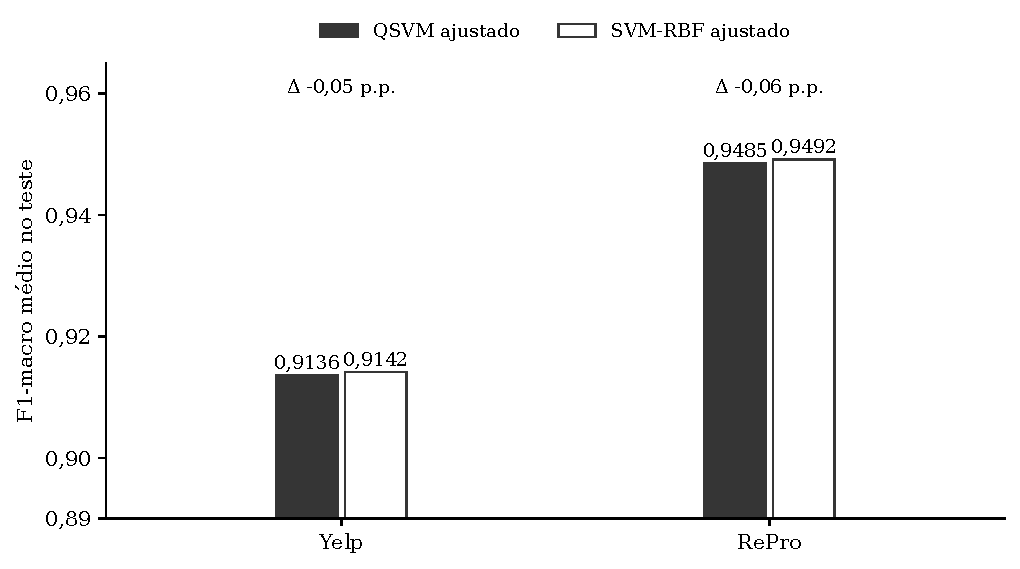
\includegraphics[width=0.8\textwidth]{figuras/fig_principal.pdf}
\caption{F1-macro médio de teste do QSVM e do \svm{} ajustados no cenário exato, por base. Cada barra representa a média das seis configurações de compressão e número de qubits, com 10 seeds e 5 folds por configuração. O eixo vertical começa em 0,89. $\Delta$ é a diferença QSVM menos \svm{}, em pontos percentuais. A figura é descritiva; os intervalos de confiança e p-valores por configuração estão na Tabela~\ref{tab:testes}.}
\label{fig:principal}
\end{figure*}

\subsection{Comparação principal e comparativo base (H\textsubscript{0} a H\textsubscript{2})}
A Tabela~\ref{tab:testes} mostra os testes pareados da comparação principal no cenário exato; os testes completos das demais comparações estão no material suplementar. Nenhuma das 12 diferenças entre o QSVM ajustado e o \svm{} ajustado foi significativa, nem antes da correção de Holm, com p-valores a partir de 0,57 e diferenças médias entre $-0{,}003$ e $+0{,}001$, e por isso H\textsubscript{0} não é rejeitada. Os intervalos de confiança ficaram entre $-0{,}013$ e $+0{,}010$, e a diferença com cerca de 80\% de chance de ser detectada ficou entre 0,015 e 0,020, dependendo da configuração. Também não houve diferença significativa entre o \svm{} ajustado e o \svm{} padrão (p-valores a partir de 0,46, com diferenças entre $-0{,}002$ e $+0{,}004$), nem entre o QSVM e o \svm{} padrão (a partir de 0,38) ou entre o QSVM e a regressão logística (a partir de 0,19). Na rodada anterior, em que a busca não era aninhada, o \svm{} ajustado ficava abaixo do \svm{} padrão nas configurações com NCA; nesta rodada, isso deixou de acontecer, e as diferenças a favor do QSVM que apareciam nessas configurações também desapareceram.

\begin{table*}[t]
\centering
\caption{Comparação principal entre QSVM e SVM ajustados no cenário exato, com 50 diferenças pareadas por configuração: diferença média de F1-macro com intervalo de confiança de 95\%, estatística $t$ corrigida de Nadeau e Bengio (49 graus de liberdade), p-valor com correção de Holm sobre as 12 configurações da comparação principal e diferença com cerca de 80\% de chance de ser detectada (DMD). Valores são arredondados; linhas iguais na tabela podem diferir antes do arredondamento.}
\label{tab:testes}
\footnotesize
\begin{tabular}{lllccccc}
\toprule
Comparação & Base & Compr. & $d$ & $\Delta$ F1 [IC 95\%] & $t$ & $p_{\mathrm{Holm}}$ & DMD \\
\midrule
H\textsubscript{1}: QSVM aj. $-$ SVM aj. & Yelp & PCA & 4 & 0,000 [-0,010; 0,010] & 0,04 & 1,000 & 0,019 \\
 & Yelp & PCA & 8 & 0,000 [-0,008; 0,008] & 0,02 & 1,000 & 0,016 \\
 & Yelp & PCA & 12 & -0,001 [-0,011; 0,009] & -0,17 & 1,000 & 0,020 \\
 & Yelp & NCA & 4 & 0,000 [-0,007; 0,008] & 0,05 & 1,000 & 0,015 \\
 & Yelp & NCA & 8 & -0,001 [-0,009; 0,007] & -0,20 & 1,000 & 0,016 \\
 & Yelp & NCA & 12 & -0,002 [-0,012; 0,008] & -0,37 & 1,000 & 0,020 \\
 & RePro & PCA & 4 & 0,001 [-0,007; 0,010] & 0,32 & 1,000 & 0,017 \\
 & RePro & PCA & 8 & 0,000 [-0,010; 0,009] & -0,04 & 1,000 & 0,018 \\
 & RePro & PCA & 12 & -0,003 [-0,013; 0,007] & -0,58 & 1,000 & 0,019 \\
 & RePro & NCA & 4 & 0,001 [-0,007; 0,010] & 0,32 & 1,000 & 0,017 \\
 & RePro & NCA & 8 & -0,003 [-0,012; 0,007] & -0,55 & 1,000 & 0,018 \\
 & RePro & NCA & 12 & -0,001 [-0,010; 0,008] & -0,25 & 1,000 & 0,017 \\
\bottomrule
\end{tabular}
\end{table*}

\subsection{Efeito da compressão (H\textsubscript{3})}
A Tabela~\ref{tab:h3} mostra a diferença média entre o QSVM e o \svm{} ajustado com PCA e com NCA. Como a H\textsubscript{3} prevê uma diferença menor em magnitude com NCA, é preciso separar duas coisas. O teste da tabela compara a diferença assinada entre as duas compressões, e essa mudança não foi significativa em nenhuma configuração (p-valores a partir de 0,73 antes da correção de Holm). Em termos descritivos, a magnitude da diferença ficou abaixo de 0,003 nas duas compressões. Como o teste compara as diferenças assinadas, ele não testa diretamente se a magnitude da diferença diminuiu com NCA.

\begin{table}[t]
\centering
\caption{H\textsubscript{3}: diferença média de F1-macro entre QSVM ajustado e SVM ajustado com PCA e com NCA, no cenário exato, e p-valor do $t$ corrigido para a mudança dessa diferença entre as duas compressões, com correção de Holm sobre as 6 configurações.}
\label{tab:h3}
\footnotesize
\begin{tabular}{lcccc}
\toprule
Base & $d$ & $\Delta$ PCA & $\Delta$ NCA & $p_{\mathrm{Holm}}$ \\
\midrule
Yelp & 4 & 0,000 & 0,000 & 1,000 \\
Yelp & 8 & 0,000 & -0,001 & 1,000 \\
Yelp & 12 & -0,001 & -0,002 & 1,000 \\
RePro & 4 & 0,001 & 0,001 & 1,000 \\
RePro & 8 & 0,000 & -0,003 & 1,000 \\
RePro & 12 & -0,003 & -0,001 & 1,000 \\
\bottomrule
\end{tabular}
\end{table}

\subsection{Número de qubits e concentração do kernel (H\textsubscript{4})}
A variância dos valores do kernel fora da diagonal foi analisada de 2 a 16 qubits na RePro; na Yelp, os valores ficaram na mesma ordem de grandeza. Com emaranhamento e $b = 1$, a variância caiu de $5{,}3\times10^{-2}$ com 2 qubits para $1{,}6\times10^{-9}$ com 16, e com $b = 0{,}1$ ela caiu de $6{,}9\times10^{-2}$ para $5{,}1\times10^{-6}$. Com $b = 0{,}01$, a variância aumentou com o número de qubits, de $3{,}1\times10^{-5}$ para $5{,}1\times10^{-2}$. Sem emaranhamento, a variância com $b = 1$ caiu de forma bem mais lenta, de $7{,}3\times10^{-2}$ para $1{,}3\times10^{-5}$, e com as larguras menores ela aumentou com o número de qubits.

\begin{figure*}[t]
\centering
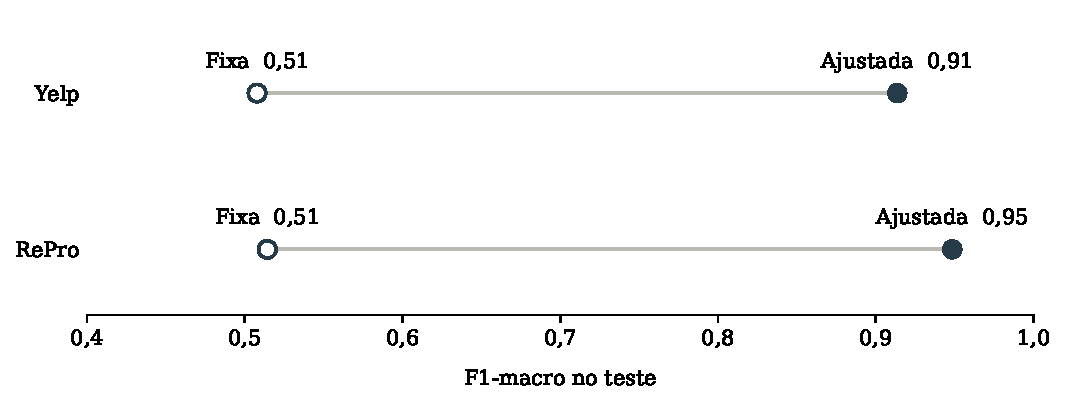
\includegraphics[width=0.55\textwidth]{figuras/fig_f1_treino_teste.pdf}
\caption{F1-macro médio de teste do QSVM com largura de banda fixa e ajustada no cenário exato. Cada ponto resume as seis configurações de compressão e número de qubits, com 10 seeds e 5 folds por configuração; os pontos são médias descritivas, sem intervalos de confiança. Os valores por configuração estão na Tabela~\ref{tab:f1_exato}.}
\label{fig:f1_treino_teste}
\end{figure*}

Na Fig.~\ref{fig:f1_treino_teste}, o F1-macro de teste é apresentado para as duas configurações de largura. No experimento de classificação, a diferença entre o QSVM com largura ajustada e o QSVM com largura fixa foi significativa em todas as 12 configurações, de $+0{,}39$ a $+0{,}45$. A Tabela~\ref{tab:treino_alinhamento} mostra que, com largura fixa e 8 ou 12 qubits, o F1-macro no treino foi 1,000 e no teste ficou perto de 0,50, enquanto com 4 qubits o F1-macro no treino ficou em torno de 0,77, também com o teste perto de 0,50. Com a largura ajustada, o valor escolhido diminuiu conforme o número de qubits aumentou, ficando principalmente entre 0,01 e 0,02 com 4 qubits, entre 0,005 e 0,01 com 8 e entre 0,001 e 0,005 com 12, e o menor valor da grade (0,0005) foi escolhido em no máximo 2\% dos folds. Com esse ajuste, não houve queda consistente do F1-macro do QSVM entre 4 e 12 qubits.

\begin{table}[t]
\centering
\caption{F1-macro no treino e no teste do QSVM com largura de banda fixa ($b = 1$) e alinhamento centrado entre o kernel quântico escolhido e o kernel RBF do \svm{} ajustado, no cenário exato (médias entre seeds e folds).}
\label{tab:treino_alinhamento}
\footnotesize
\resizebox{\columnwidth}{!}{%
\begin{tabular}{llccccc}
\toprule
& & & \multicolumn{2}{c}{QSVM largura fixa} & \multicolumn{2}{c}{Alinhamento com RBF} \\
Base & Compr. & $d$ & treino & teste & QSVM aj. & QSVM sep. \\
\midrule
Yelp & PCA & 4 & 0,771 & 0,519 & 0,694 & 0,941 \\
Yelp & PCA & 8 & 1,000 & 0,504 & 0,434 & 0,966 \\
Yelp & PCA & 12 & 1,000 & 0,497 & 0,383 & 0,959 \\
Yelp & NCA & 4 & 0,776 & 0,523 & 0,706 & 0,953 \\
Yelp & NCA & 8 & 1,000 & 0,506 & 0,439 & 0,984 \\
Yelp & NCA & 12 & 1,000 & 0,499 & 0,397 & 0,976 \\
\midrule
RePro & PCA & 4 & 0,769 & 0,517 & 0,703 & 0,943 \\
RePro & PCA & 8 & 1,000 & 0,504 & 0,427 & 0,956 \\
RePro & PCA & 12 & 1,000 & 0,523 & 0,383 & 0,974 \\
RePro & NCA & 4 & 0,767 & 0,511 & 0,699 & 0,950 \\
RePro & NCA & 8 & 1,000 & 0,516 & 0,445 & 0,962 \\
RePro & NCA & 12 & 1,000 & 0,514 & 0,404 & 0,954 \\
\bottomrule
\end{tabular}}
\end{table}

A Tabela~\ref{tab:treino_alinhamento} também mostra o alinhamento centrado entre o kernel quântico escolhido e o kernel RBF do \svm{} ajustado. Para o QSVM ajustado, ele ficou em torno de 0,70 com 4 qubits e caiu para valores entre 0,38 e 0,45 com 8 e 12 qubits, enquanto para o QSVM sem emaranhamento ficou entre 0,94 e 0,98 em todas as configurações.

\subsection{Shots e ruído}
A Tabela~\ref{tab:cenarios} mostra o QSVM ajustado nos diferentes cenários. Em relação ao estado exato, a estimativa com 1.000 shots reduziu o F1-macro em 0,002 a 0,008 com 4 qubits, em 0,008 a 0,013 com 8 e em 0,011 a 0,015 com 12. Com ruído de $p = 0{,}001$, a redução foi de 0,004 a 0,011 com 4 qubits e de 0,012 a 0,015 com 8, e com $p = 0{,}01$ ela foi de 0,008 a 0,013 com 4 qubits e de 0,069 a 0,089 com 8, configuração em que o fator $F$ fica em 0,105. Com shots e com ruído de $p = 0{,}001$, nenhuma diferença entre o QSVM ajustado e os modelos clássicos foi significativa. Com $p = 0{,}01$ e 8 qubits, o QSVM ficou significativamente abaixo do \svm{} ajustado, do \svm{} padrão, da regressão logística e da versão sem emaranhamento nas 4 configurações, com diferenças de $-0{,}065$ a $-0{,}090$; com 4 qubits, nenhuma dessas diferenças foi significativa. A versão sem emaranhamento, que não tem CNOTs, ficou entre 0,908 e 0,950 nesse mesmo cenário.

\begin{table}[t]
\centering
\caption{F1-macro do QSVM ajustado em cada cenário de cálculo do kernel. Os cenários com ruído foram rodados só com 4 e 8 qubits.}
\label{tab:cenarios}
\footnotesize
\resizebox{\columnwidth}{!}{%
\begin{tabular}{llccccc}
\toprule
Base & Compr. & $d$ & Exato & 1.000 shots & Ruído $p=0{,}001$ & Ruído $p=0{,}01$ \\
\midrule
Yelp & PCA & 4 & 0,917 & 0,910 & 0,907 & 0,906 \\
Yelp & PCA & 8 & 0,917 & 0,906 & 0,904 & 0,828 \\
Yelp & PCA & 12 & 0,914 & 0,899 & n.a. & n.a. \\
Yelp & NCA & 4 & 0,911 & 0,904 & 0,904 & 0,897 \\
Yelp & NCA & 8 & 0,911 & 0,903 & 0,899 & 0,834 \\
Yelp & NCA & 12 & 0,912 & 0,902 & n.a. & n.a. \\
\midrule
RePro & PCA & 4 & 0,942 & 0,934 & 0,931 & 0,929 \\
RePro & PCA & 8 & 0,953 & 0,941 & 0,939 & 0,876 \\
RePro & PCA & 12 & 0,952 & 0,938 & n.a. & n.a. \\
RePro & NCA & 4 & 0,947 & 0,945 & 0,943 & 0,939 \\
RePro & NCA & 8 & 0,948 & 0,937 & 0,933 & 0,879 \\
RePro & NCA & 12 & 0,949 & 0,935 & n.a. & n.a. \\
\bottomrule
\end{tabular}}
\end{table}

\subsection{Ablação sem emaranhamento (H\textsubscript{5})}
No cenário exato, nenhuma diferença entre o QSVM com e sem emaranhamento foi significativa (p-valores a partir de 0,69, com diferenças entre $-0{,}002$ e $+0{,}002$), e o mesmo aconteceu com 1.000 shots e com ruído de $p = 0{,}001$. Com ruído de $p = 0{,}01$ e 8 qubits, a versão com emaranhamento ficou abaixo, como descrito acima.

\subsection{Descrição objetiva dos resultados}
Nos experimentos realizados, (i) os modelos clássicos chegaram a valores entre 0,91 e 0,95 de F1-macro já com 4 dimensões, nas duas bases; (ii) com a largura de banda ajustada, o QSVM ficou entre 0,91 e 0,95 em todas as dimensões, sem diferença significativa em relação ao \svm{} ajustado, ao \svm{} padrão, à regressão logística e à versão sem emaranhamento no cenário exato; (iii) a compressão com NCA não mudou de forma significativa a diferença entre o QSVM e o \svm{}; (iv) com largura de banda fixa, o QSVM decorou o treino com 8 e 12 qubits e ficou perto de 0,50 no teste, enquanto, com a largura ajustada, os valores escolhidos diminuíram com o número de qubits; (v) o kernel quântico ajustado teve alinhamento entre 0,38 e 0,70 com o kernel RBF, e o kernel sem emaranhamento, entre 0,94 e 0,98; e (vi) a redução de F1-macro com shots e ruído aumentou com o número de qubits, e o ruído de $p = 0{,}01$ deixou o QSVM com 8 qubits significativamente abaixo dos demais modelos. O mesmo padrão apareceu nas duas bases.

\FloatBarrier
\section{Discussão}
\label{sec:discussao}

\subsection{Análise das hipóteses e dos objetivos}
A Tabela~\ref{tab:hipoteses} resume o que os resultados dizem sobre cada hipótese. O resultado central é que, quando o QSVM e os modelos clássicos recebem as mesmas features comprimidas e passam pelo mesmo procedimento de ajuste, nenhuma diferença foi detectada entre eles no cenário exato, e isso vale para as duas bases e para as duas formas de compressão. A diferença com cerca de 80\% de chance de ser detectada foi estimada entre 0,015 e 0,020, conforme a configuração. Essa estimativa indica a sensibilidade aproximada dos testes, mas diferenças reais, inclusive dessa ordem ou maiores, podem não ter sido detectadas.

\begin{table}[t]
\centering
\caption{Resumo das hipóteses no cenário de estado exato.}
\label{tab:hipoteses}
\footnotesize
\setlength{\tabcolsep}{3pt}
\begin{tabular}{>{\raggedright\arraybackslash}p{0.13\columnwidth}>{\raggedright\arraybackslash}p{0.22\columnwidth}>{\raggedright\arraybackslash}p{0.55\columnwidth}}
\toprule
Hipótese & Resultado & Evidência \\
\midrule
H\textsubscript{0}/H\textsubscript{1} & H\textsubscript{0} não rejeitada & nenhuma das 12 diferenças entre QSVM e \svm{} ajustado foi significativa \\
H\textsubscript{2} & não confirmada & não foram detectadas diferenças significativas entre os modelos nessas comparações \\
H\textsubscript{3} & não avaliada diretamente & o teste não detectou mudança significativa na diferença assinada; a hipótese trata da magnitude \\
H\textsubscript{4} & parcialmente confirmada & com largura fixa, a variância cai e o QSVM decora o treino com 8 e 12 qubits; com largura ajustada, não há queda consistente, mas o QSVM já está no acaso com 4 qubits, então a queda ao longo das dimensões não aparece \\
H\textsubscript{5} & não contrariada & não foi detectada diferença significativa entre as versões com e sem emaranhamento \\
\bottomrule
\end{tabular}
\end{table}

Em relação aos objetivos, o estudo realizou as comparações e análises propostas, com a ressalva de que a H\textsubscript{3} não foi testada diretamente em termos de magnitude. O pipeline foi montado com a compressão e a busca de hiperparâmetros totalmente aninhadas; o QSVM foi comparado com a regressão logística, com o \svm{} e com a versão sem emaranhamento; o efeito do ajuste do \svm{} e o da compressão com e sem rótulos foram testados; o comportamento do kernel com o número de qubits foi analisado na simulação exata e com medições finitas; o efeito do ruído foi avaliado com 4 e 8 qubits; e o código e as configurações estão disponíveis no repositório descrito na Seção~\ref{sec:codigo}.

\subsection{Por que o QSVM fica no mesmo patamar dos modelos clássicos}
A regressão logística, que é um modelo linear, teve a maior média ou ficou a menos de 0,003 da maior em todas as configurações e não teve diferença significativa em relação ao QSVM ajustado, que foi a única comparação testada para ela. Isso sugere que, depois da compressão, a tarefa é quase linear, o que deixa pouco espaço para que um kernel, quântico ou clássico, mostre vantagem. O alinhamento entre os kernels ajuda a completar essa leitura. O kernel sem emaranhamento ficou muito parecido com o kernel RBF escolhido para o \svm{}, com alinhamento acima de 0,94, mas o kernel com emaranhamento ficou bem menos parecido, principalmente com 8 e 12 qubits, e, mesmo assim, não foi detectada diferença significativa de desempenho. Ou seja, os resultados não confirmam a ideia de que o kernel quântico simplesmente se transforma no kernel RBF com larguras pequenas. Os resultados mostram desempenhos próximos para kernels diferentes, o que é compatível com uma tarefa em que a fronteira entre as classes é simples.

A comparação com a rodada anterior deste mesmo estudo reforça o ponto que motivou o trabalho. Na rodada 2, com a busca de hiperparâmetros sem aninhamento, o \svm{} ajustado ficava abaixo do \svm{} padrão nas configurações com NCA, e era justamente nelas que o QSVM aparecia com as maiores diferenças a favor, ainda que não significativas. Na rodada 3, essas diferenças desapareceram. Entre as duas rodadas, mudaram principalmente o aninhamento da busca, mas também a grade de largura de banda e, na Yelp, a remoção das frases repetidas. Para o \svm{} na RePro, porém, só o aninhamento mudou, já que os dados e a grade do \svm{} são os mesmos, e ali o \svm{} ajustado também deixou de ficar abaixo do padrão. Isso indica que uma escolha de hiperparâmetros enviesada no comparativo base pode ser suficiente para criar uma aparente vantagem do QSVM, que é o tipo de efeito que a introdução descreve nos trabalhos relacionados.

\subsection{Largura de banda, shots e ruído}
O comportamento com largura fixa mostra o que acontece quando o kernel concentra. Com 8 e 12 qubits e $b = 1$, o QSVM acertou todo o treino e ficou perto de 0,50 no teste, ou seja, decorou os exemplos, já que, nessas condições, o kernel fica muito próximo da matriz identidade. Com 4 qubits, o QSVM nem decorou o treino nem generalizou, o que indica que, nessa largura, o kernel também não captura a estrutura dos dados, mesmo sem estar tão concentrado. Com a largura ajustada, a busca escolheu valores cada vez menores conforme os qubits aumentaram, e isso evitou a queda de desempenho, como esperado a partir de Shaydulin e Wild \cite{shaydulin2021}.

Esse ajuste, porém, tem um custo quando o kernel é estimado com medições finitas. Com larguras pequenas, os valores do kernel ficam perto de 1, então as diferenças entre eles ficam pequenas perto do erro dos shots, o que ajuda a explicar por que a redução de F1-macro com 1.000 shots aumentou com o número de qubits. Com ruído de $p = 0{,}01$ e 8 qubits, o fator $F$ encolhe ainda mais essas diferenças, e a queda chegou a quase 0,09. Como a versão sem emaranhamento não tem CNOTs, o modelo de ruído usado não a afeta, e ela manteve o desempenho, mas isso vem da forma como o ruído foi modelado e não significa que um circuito sem emaranhamento estaria livre de erros em hardware.

\subsection{Compressão e língua}
Olhando só as médias, sem um teste específico para isso, a NCA não trouxe melhora consistente sobre o PCA. Com PCA e só 4 dimensões, os modelos clássicos já chegaram a 0,92 na Yelp e a 0,94 na RePro. Como nenhum modelo foi treinado com os 384 componentes originais, não é possível dizer quanto a compressão perdeu, mas esses valores são altos para uma representação tão pequena, diferente do que Hassan et al. \cite{hassan2026} observaram em uma tarefa de 6 classes, em que o PCA perdia bastante informação. Uma possível explicação, que não foi testada aqui, é que, como a tarefa é binária, o sentimento fique concentrado nas primeiras direções do embedding. Em relação à língua, o padrão foi o mesmo nas duas bases, o que sugere que a conclusão sobre a comparação entre os modelos se mantém em outra língua e em outro domínio, dentro do que foi testado.

\subsection{Comparação com trabalhos relacionados}
A Tabela~\ref{tab:comparacao} coloca os principais resultados deste trabalho ao lado do que os trabalhos relacionados relataram. De forma geral, os resultados vão na mesma direção dos estudos que fizeram comparações mais controladas \cite{bowles2024,kolle2024} e não reproduzem, com embeddings de texto, o ganho relatado contra um SVM com hiperparâmetros fixos \cite{cajas2025}. Como as tarefas, os dados e os circuitos são diferentes, isso não mostra que os resultados desses trabalhos estejam errados, e sim que, no cenário avaliado aqui, a vantagem não apareceu.

\begin{table*}[t]
\centering
\caption{Comparação entre o que os trabalhos relacionados relataram e o que foi observado neste trabalho.}
\label{tab:comparacao}
\footnotesize
\begin{tabular}{p{0.16\textwidth}p{0.38\textwidth}p{0.38\textwidth}}
\toprule
Trabalho & O que relatou & O que foi observado aqui \\
\midrule
Bowles et al. \cite{bowles2024} & modelos clássicos superaram os quânticos de forma geral, e retirar o emaranhamento não piorou o desempenho & QSVM no mesmo patamar dos clássicos sem diferença significativa detectada em relação à versão sem emaranhamento \\
Kölle et al. \cite{kolle2024} & em modelos híbridos, a parte clássica faz boa parte do trabalho & a compressão clássica seguida de uma regressão logística já chega ao melhor desempenho \\
Hassan et al. \cite{hassan2026} & compressão de embeddings de texto antes de um VQC, sem clássico nas mesmas features, e perda grande com PCA em 6 classes & com o clássico nas mesmas features, não houve diferença significativa detectada, e o PCA com 4 dimensões já chegou a 0,92 e 0,94 na tarefa binária \\
Cajas Ordóñez et al. \cite{cajas2025} & ganho relativo de até 8\% do kernel quântico sobre um SVM com hiperparâmetros fixos, em embeddings de imagens & com embeddings de texto, o QSVM não superou o SVM padrão em nenhuma configuração \\
Djemmal et al. \cite{djemmal2025} & QNN com PCA perto de 50\% de acurácia, prevendo praticamente uma classe & QSVM com PCA entre 0,91 e 0,95, o que sugere que o desempenho baixo com PCA não é inevitável \\
Thanasilp et al. \cite{thanasilp2024} e Shaydulin e Wild \cite{shaydulin2021} & concentração do kernel com o aumento de qubits, evitada com o ajuste da largura de banda & concentração e memorização com largura fixa, e desempenho mantido com a largura ajustada \\
\bottomrule
\end{tabular}
\end{table*}

\subsection{Limitações}
O teste $t$ corrigido reduz o efeito da dependência entre os folds, mas continua sendo uma aproximação, e diferenças menores que algo entre 0,015 e 0,020 podem não ter sido detectadas; a ausência de diferença significativa também não demonstra que os modelos são equivalentes. O kernel foi simulado e não executado em hardware, e o ruído segue um modelo de despolarização global, que é uma simplificação forte do ruído real. Foi usado um único modelo de embedding, um único feature map e duas bases pequenas, que diferem também no domínio e no tamanho dos textos. Na RePro, avaliações de um mesmo produto podem aparecer no treino e no teste, pois os folds foram formados por avaliação. Assim, os resultados não medem especificamente a generalização para produtos inéditos. As grades de hiperparâmetros são finitas, e, embora a largura escolhida tenha ficado no limite inferior em poucos folds, outros valores fora da grade não foram testados. Além disso, o alinhamento foi medido só em relação ao kernel RBF escolhido para o \svm{}, e não em relação a outras formas de kernel clássico. Por isso, os resultados devem ser lidos como evidência para esse cenário, e não como uma conclusão geral sobre kernels quânticos.

\begin{table}[t]
\centering
\caption{Organização do repositório.}
\label{tab:codigo}
\footnotesize
\begin{tabular}{p{0.46\columnwidth}p{0.44\columnwidth}}
\toprule
Arquivo ou pasta & Função \\
\midrule
\texttt{config.py} & todos os parâmetros do experimento \\
\texttt{01\_preparar\_dados.py} & seleção das bases e estatísticas de tamanho \\
\texttt{02\_gerar\_embeddings.py} & embeddings com o modelo multilíngue \\
\texttt{quantico.py} & simulação do ZZ feature map, shots e ruído \\
\texttt{validar\_qiskit.py} & comparação da simulação com o Qiskit \\
\texttt{03\_rodar\_experimentos.py} & validação cruzada aninhada, ajuste e treino \\
\texttt{04\_concentracao.py} & variância e alinhamento do kernel \\
\texttt{05\_estatistica.py} & teste $t$ corrigido e correção de Holm \\
\texttt{06\_tabelas\_latex.py} & tabelas do artigo \\
\texttt{07\_figuras.py} & figuras do artigo \\
\texttt{dados/}, \texttt{resultados/} & bases, embeddings e resultados por fold \\
\bottomrule
\end{tabular}
\end{table}

\section{Conclusão}
\label{sec:conclusao}

Este trabalho comparou um QSVM com kernel quântico de fidelidade a classificadores clássicos sobre as mesmas representações comprimidas de textos em português e inglês, com todos os modelos ajustados pelo mesmo procedimento aninhado. Respondendo à pergunta principal, não foi detectada diferença estatisticamente significativa entre o QSVM e o \svm{} ajustado em nenhuma das 12 configurações no cenário exato, e o mesmo valeu para o \svm{} padrão, a regressão logística e a versão do circuito sem emaranhamento. Permitir o ajuste da largura de banda esteve associado a uma grande diferença de desempenho: com largura fixa, o QSVM ficou perto de 0,50 no teste e, com 8 e 12 qubits, decorou o treino. Nesse contraste, o valor de C também podia mudar. As medições finitas e o ruído reduziram mais o desempenho conforme o número de qubits aumentou.

Além da comparação em si, o estudo mostrou, dentro dos seus próprios experimentos, como as condições da comparação mudam a conclusão, já que as diferenças aparentes a favor do QSVM que surgiam com a busca de hiperparâmetros sem aninhamento sumiram quando o procedimento foi corrigido, junto com os outros ajustes da última rodada. Para trabalhos que comparam modelos quânticos e clássicos, isso reforça a importância de usar as mesmas features, o mesmo procedimento de ajuste e testes estatísticos que levem em conta a dependência entre os folds.

\subsection{Trabalhos futuros}
Algumas extensões ficam para trabalhos futuros. Uma validação com folds agrupados por produto permitiria avaliar a generalização para produtos não vistos durante o treino. Um teste de equivalência, com uma margem definida antes dos experimentos, permitiria dizer se os modelos são de fato equivalentes, e não só que nenhuma diferença foi detectada. Também vale testar outros feature maps, kernels com parâmetros treináveis e compressões aprendidas, como a de Djemmal et al. \cite{djemmal2025}, dentro do mesmo protocolo pareado, além de outros modelos de embedding, mais bases em português e tarefas com mais classes, como a de Hassan et al. \cite{hassan2026}. Por fim, executar as configurações menores em hardware real e usar modelos de ruído calibrados com dados de dispositivos mostraria se o efeito do ruído observado aqui se mantém fora da simulação.

\FloatBarrier
\section{Organização dos códigos e dados}
\label{sec:codigo}

O código está organizado em scripts numerados, que rodam em sequência e salvam tudo o que é usado no artigo (Tabela~\ref{tab:codigo}). Todos os parâmetros ficam em um único arquivo (\texttt{config.py}), os resultados de cada fold ficam em CSV com os hiperparâmetros escolhidos, o F1-macro no treino e o alinhamento com o kernel RBF, e as tabelas e figuras do artigo são geradas direto a partir desses arquivos. O experimento principal salva o resultado ao fim de cada combinação de base e seed, o que permite dividir a execução em vários processos e retomar de onde parou se for interrompido. As versões das bibliotecas usadas estão fixadas no arquivo de dependências. O repositório está disponível em \url{https://github.com/julialveszz/kernel-quantico-sentimentos}, e os resultados das duas primeiras rodadas, com as grades de largura de banda anteriores e a busca sem aninhamento, ficaram guardados em \texttt{resultados/rodada1/} e \texttt{resultados/rodada2/}. A Yelp é distribuída sob a licença CC BY 4.0 e a RePro sob a CC BY-NC-SA 4.0, que permite o uso acadêmico.



\begin{thebibliography}{00}
\bibitem{reimers2019} N. Reimers e I. Gurevych, ``Sentence-BERT: Sentence embeddings using Siamese BERT-networks,'' in \textit{Proc. EMNLP-IJCNLP}, 2019.
\bibitem{havlicek2019} V. Havl\'{\i}\v{c}ek, A. D. C\'{o}rcoles, K. Temme, A. W. Harrow, A. Kandala, J. M. Chow e J. M. Gambetta, ``Supervised learning with quantum-enhanced feature spaces,'' \textit{Nature}, vol. 567, pp. 209-212, 2019.
\bibitem{bowles2024} J. Bowles, S. Ahmed e M. Schuld, ``Better than classical? The subtle art of benchmarking quantum machine learning models,'' arXiv:2403.07059, 2024.
\bibitem{hassan2026} A. Hassan, Z. Zhao e M. A. Metawei, ``Hybrid quantum-classical NLP classification with compact semantic representations: An experimental analysis of representation compression,'' arXiv:2609.10089, 2026.
\bibitem{kolle2024} M. Kölle et al., ``Disentangling quantum and classical contributions in hybrid quantum machine learning architectures,'' arXiv:2311.05559, 2023 (rev. 2024).
\bibitem{cajas2025} S. A. Cajas Ord\'{o}\~{n}ez, L. F. Torres Torres, M. Bifulco, C. A. Dur\'{a}n, C. Bosch e R. Sim\'{o}n Carbajo, ``Embedding-aware quantum-classical SVMs for scalable quantum machine learning,'' in \textit{Proc. 3rd Int. Workshop on AI for Quantum and Quantum for AI (AIQxQIA 2025)}, CEUR Workshop Proceedings, vol. 4153, 2026.
\bibitem{djemmal2025} I. Djemmal, H. Belhadef e A. M. Mutawa, ``Neural quantum embedding enhanced hybrid quantum-classical sentiment analysis classification,'' preprint, Research Square, rs-8197450/v1, 2025.
\bibitem{thanasilp2024} S. Thanasilp, S. Wang, M. Cerezo e Z. Holmes, ``Exponential concentration in quantum kernel methods,'' \textit{Nature Communications}, vol. 15, 2024.
\bibitem{shaydulin2021} R. Shaydulin e S. M. Wild, ``Importance of kernel bandwidth in quantum machine learning,'' arXiv:2111.05451, 2021.
\bibitem{maio2026} D. Maio, ``On the representational limits of quantum-inspired 1024-D document embeddings: An experimental evaluation framework,'' arXiv:2604.09430, 2026.
\bibitem{kotzias2015} D. Kotzias, M. Denil, N. de Freitas e P. Smyth, ``From group to individual labels using deep features,'' in \textit{Proc. ACM SIGKDD}, pp. 597-606, 2015.
\bibitem{repro2024} L. N. dos Santos Silva, L. Real, A. C. B. Zandavalle, C. F. G. Rodrigues, T. da Silva Gama, F. G. Souza e P. D. S. Zaidan, ``RePro: a benchmark for opinion mining for Brazilian Portuguese,'' in \textit{Proc. PROPOR}, pp. 432-440, 2024.
\bibitem{real2019} L. Real, M. Oshiro e A. Mafra, ``B2W-Reviews01: an open product reviews corpus,'' in \textit{Proc. STIL}, 2019.
\bibitem{reimers2020} N. Reimers e I. Gurevych, ``Making monolingual sentence embeddings multilingual using knowledge distillation,'' in \textit{Proc. EMNLP}, 2020.
\bibitem{jolliffe2002} I. T. Jolliffe, \textit{Principal Component Analysis}, 2. ed. New York: Springer, 2002.
\bibitem{goldberger2004} J. Goldberger, S. Roweis, G. Hinton e R. Salakhutdinov, ``Neighbourhood components analysis,'' in \textit{Advances in Neural Information Processing Systems 17}, 2004.
\bibitem{cortes1995} C. Cortes e V. Vapnik, ``Support-vector networks,'' \textit{Machine Learning}, vol. 20, no. 3, pp. 273-297, 1995.
\bibitem{schuld2019} M. Schuld e N. Killoran, ``Quantum machine learning in feature Hilbert spaces,'' \textit{Physical Review Letters}, vol. 122, 040504, 2019.
\bibitem{djemmal2025arabert} I. Djemmal e H. Belhadef, ``AraBERT-QC: a novel quantum-based classification architecture to classify short Arabic sentences,'' \textit{The Journal of Supercomputing}, vol. 81, 1466, 2025.
\bibitem{masum2023} A. K. M. Masum, A. Maurya, D. S. Murthy, Pratibha e N. Mahmud, ``Hybrid quantum-classical machine learning for sentiment analysis,'' in \textit{Proc. ICMLA}, pp. 1006-1011, 2023.
\bibitem{pedregosa2011} F. Pedregosa et al., ``Scikit-learn: Machine learning in Python,'' \textit{Journal of Machine Learning Research}, vol. 12, pp. 2825-2830, 2011.
\bibitem{qiskit2024} A. Javadi-Abhari et al., ``Quantum computing with Qiskit,'' arXiv:2405.08810, 2024.
\bibitem{cortes2012} C. Cortes, M. Mohri e A. Rostamizadeh, ``Algorithms for learning kernels based on centered alignment,'' \textit{Journal of Machine Learning Research}, vol. 13, pp. 795-828, 2012.
\bibitem{cristianini2001} N. Cristianini, J. Shawe-Taylor, A. Elisseeff e J. Kandola, ``On kernel-target alignment,'' in \textit{Advances in Neural Information Processing Systems 14}, 2001.
\bibitem{nadeau2003} C. Nadeau e Y. Bengio, ``Inference for the generalization error,'' \textit{Machine Learning}, vol. 52, no. 3, pp. 239-281, 2003.
\bibitem{bouckaert2004} R. R. Bouckaert e E. Frank, ``Evaluating the replicability of significance tests for comparing learning algorithms,'' in \textit{Proc. PAKDD}, pp. 3-12, 2004.
\bibitem{holm1979} S. Holm, ``A simple sequentially rejective multiple test procedure,'' \textit{Scandinavian Journal of Statistics}, vol. 6, no. 2, pp. 65-70, 1979.
\end{thebibliography}

\end{document}
